\documentclass[mat1, tisk]{fmfdelo}
% \documentclass[fin1, tisk]{fmfdelo}
% Če pobrišete možnost tisk, bodo povezave obarvane,
% na začetku pa ne bo praznih strani po naslovu, …

%%%%%%%%%%%%%%%%%%%%%%%%%%%%%%%%%%%%%%%%%%%%%%%%%%%%%%%%%%%%%%%%%%%%%%%%%%%%%%%
% METAPODATKI
%%%%%%%%%%%%%%%%%%%%%%%%%%%%%%%%%%%%%%%%%%%%%%%%%%%%%%%%%%%%%%%%%%%%%%%%%%%%%%%
% - vaše ime
\avtor{Neža Kržan}
% - naslov dela v slovenščini
\naslov{Statistika v kazenskem pravu}
% - naslov dela v angleščini
\title{Criminal justice statistics}
% - ime mentorja/mentorice s polnim nazivom:
\mentor{izr. prof. dr. Jaka Smrekar}

% - leto diplome
\letnica{2023} 

% - povzetek v slovenščini
%   V povzetku na kratko opišite vsebinske rezultate dela. Sem ne sodi razlaga
%   organizacije dela, torej v katerem razdelku je kaj, pač pa le opis vsebine.
\povzetek{V diplomski nalogi se bom osredotočila na statistiko v kazenskem pravu in na zmote, ki se pojavljajo pri uporabi le te, zaradi pomanjkanja
znanja statistike pri odvetnikih, sodnikih in poroti. Osredotočila se bom na uporabo Bayesove statistike v kazenskih postopkih oziroma na izračune,
ki izhajajo iz Bayesove statistike in jo primerjala z drugimi metodami. V nadaljevanju bom opisala in razložila dve najpogostejši zmoti, prva
je Tožilčeva zmota, ki je dobro znan statistični problem, druga večja, ki pa izhaja iz prve, pa je Zmota obrambnega odvetnika. Ker je uporaba
statistike in verjetnostnega računa čedalje pogostejša v sodnih postopkih, bom na koncu pregledala resničen primer sodbe medicinski sestri Lucii de Berk.
}

% - povzetek v angleščini
\abstract{...}

% - klasifikacijske oznake, ločene z vejicami
%   Oznake, ki opisujejo področje dela, so dostopne na strani https://www.ams.org/msc/
\klasifikacija{..., ...}

% - ključne besede, ki nastopajo v delu, ločene s \sep
\kljucnebesede{...\sep ...}

% - angleški prevod ključnih besed
\keywords{...\sep ...} % angleški prevod ključnih besed

% - angleško-slovenski slovar strokovnih izrazov
\slovar{
% \geslo{angleški izraz}{slovenski izraz}
% ...
}

% - ime datoteke z viri (vključno s končnico .bib), če uporabljate BibTeX
% \literatura{....bib}

%%%%%%%%%%%%%%%%%%%%%%%%%%%%%%%%%%%%%%%%%%%%%%%%%%%%%%%%%%%%%%%%%%%%%%%%%%%%%%%
% DODATNE DEFINICIJE
%%%%%%%%%%%%%%%%%%%%%%%%%%%%%%%%%%%%%%%%%%%%%%%%%%%%%%%%%%%%%%%%%%%%%%%%%%%%%%%
\usepackage[T1]{fontenc}
\usepackage[utf8]{inputenc}
\usepackage{amsmath,amssymb,amsfonts}
\usepackage{url}
\usepackage[normalem]{ulem}
\usepackage[dvipsnames,usenames]{color}
\usepackage{graphicx}
\usepackage{lipsum}
\usepackage[slovene]{babel}

\usepackage{float}
\restylefloat{table}

% deklarirajte vse matematične operatorje, da jih bo LaTeX pravilno stavil
% \DeclareMathOperator{\...}{...}

\theoremstyle{definition} % tekst napisan pokončno
\theoremstyle{trditev} % tekst napisan pokončno
\theoremstyle{izrek}


%%%%%%%%%%%%%%%%%%%%%%%%%%%%%%%%%%%%%%%%%%%%%%%%%%%%%%%%%%%%%%%%%%%%%%%%%%%%%%%
% ZAČETEK VSEBINE
%%%%%%%%%%%%%%%%%%%%%%%%%%%%%%%%%%%%%%%%%%%%%%%%%%%%%%%%%%%%%%%%%%%%%%%%%%%%%%%

\begin{document}

V tem primeru bi lahko uporabili večina zgoraj opisanih metod in teorij - Bayesov pristop, klasični frekvenčni pristop ali 
verjetnostni pristop, ki zagovarja uporabo razmerja verjetnosti.  Vaka metoda ima lahko več rešitev za isti problem, pri čemer pa lahko nastane 
tudi vprašanje o obsegu modela.



 


Za predstavo, kako stopnje napak vplivajo na razmerje verjetnosti, predpostavim, da je pogostost profila DNK 1 proti milijardi. Predpostavim
tudi, da sta stopnji lažno poztivnih in negativnih laboratorijskih rezultatov(tj. FP in FN) enako $0,01$. Če je razmerje verjetnosti enako
$\frac{1}{f}$, je milijarda. S formulo pa dobimo:
\[
   \frac{P(M_p \lvert S)}{P(M_p \lvert \neg S)} = \frac{1 - 0,01}{[(1 - 0,01) \times 0,000000001] + [0,01 \times (1 - 0,000000001)]} \approx 99. \vspace{2mm}
\]\\
Relativno majhne stopnje napak lahko bistveno zmanjšajo dokazno vrednost DNK dokazov, saj močno zmanjšajo razmerje verjetnosti; v našem primeru
smo iz milijarde prišli na pribljižno 100. Vpliv stopnje laboratorijskih napak kaže, da ne glede na to, kako nizka se izkaže pogostost profila,
bo ta relativno nepomembna, če pogostosti ne spremlja ocena stopnje laboratorijskih napak. Bayesovo pravilo nam omogoča, da ta vidik upoštevamo.\\\\
Ker profili DNK predstavlja del naše genetske zasnove in imajo ljudje, ki so v sorodu, večjo verjetnost, da bodo imeli enak profil DNK, kot ljudje,
ki niso v sorodu morajo forenzični strokovnjaki svoje izjave vedno opredeliti z navedbo, da njihove ocene pogostosti veljajo za populacijo nepovezanih
posameznikov. To spremenljivost pogostosti profila lahko v Bayesovem okviru upoštevamo na dva načina: s spremembo predhodne verjetnosti in s
spremembo pogostosti profila. Izvedli bi lahko tudi različne izračune: enega za populacijo nepovezanih posameznikov in drugega za populacijo
sorodnih posameznikov.

%%%%%%%%%%%%%%%%%%%%%%%%%%%%%%%%%%%%%%%%%%%%%%%%%%%%%%%%%%%%%%%%%%%%%%%%%%%%%%%%%%%%%%%%%%%%%%%%%%%%%%%%%%%%%%%%%%%%%%%%%%%%%%%%%%%%%%%%%%%%%%
%%%%%%%%%%%%%%%%%%%%%%%%%%%%%%%%%%%%%%%%%%%%%%%%%%%%%%%%%%%%%%%%%%%%%%%%%%%%%%%%%%%%%%%%%%%%%%%%%%%%%%%%%%%%%%%%%%%%%%%%%%%%%%%%%%%%%%%%%%%%%%
\section{Frekvence}
Da lahko ocenilm moč Bayesove analize dokazov DNK, jo v nadaljevanju primerjam z nekaterimi drugimi pristopi. Ker je bilo predlagano s strani 
mnogih avtorjev, da je bolj naraven način za obravnavo verjetnosti uporaba naravnih frekvenc, sledi opis tega pristopa.\\\\
\begin{definicija}
   Frekvenca $f$ je posamezno število diskretnih statističnih enot iste vrednosti. Če je diskretnih podatkov zelo veliko ali če so
   podatki zvezni, jih združujemo v frekvenčne razrede.
\end{definicija}
\begin{definicija}
    Absolutna frekvenca (oznaka $f_k$ za k-ti razred) je število vrednosti statistične spremenljivke v k-tem razredu.
\end{definicija}
\begin{definicija}
    Relativna frekvenca (oznaka $f_k'$) pa je delež absolutne frekvence $f_k$ glede na celoto. Če je $N$ število enot v populaciji
    ali morda vzorcu, je
    \[
        f_k' = \frac{f_k}{N}. \vspace{2mm}
    \]
\end{definicija}
V forenzičnem kontekstu se navedene frekvence običajno nanašajo na pojavljanje dokazov za posamezen primer, medtem ko se frekvence za
pojavljanje vprašanj običajno opisujejo kot osnovne stopnje. Sklepanje o krivdi je lahko podprto s statistično analizo
ustreznih podatkov in verjetnostnim sklepanjem z uporabo absolutnih ali relativnih frekvenc, pri čemer je verjetnost, da bi določene
podatke (dokaze) pridobili zgolj po naključju, izjemno majhna. Relativne frekvence vedno navajajo ali predpostavljajo, da obstaja nek
referenčni vzorec, na podlagi katerega se lahko oceni pogostost zadevnega dogodka. Nadaljnja predpostavka je, da je ta primerjava poučna
in pomembna za obravnavano nalogo. V okviru kazenskega postopka bi na primer pričakovali, da bo relativna frekvenca lahko podprla
vmesno sklepanje o moči dokazov, ki se nanašajo na sporna dejstva, kar vodi do končnega sklepa, da je obtoženec nedolžen ali kriv. Relativne
frekvence so rutinsko vključene v znanstvene dokaze, ki se predložijo v kazenskih postopkih.\\\\
Recimo, da je pogostost profila DNK $f$ 1 proti 10 milijonov, predpostavimo tudi, da ima obtoženec enak DNK in da je začetna populacija osumljencev
100 milijonov ljudi. Zanima nas kakšna je verjetnost, da je obtoženec vir DNK-ja s kraja zločina. \\
Naj bo \\
$f$ \dots pogostost profila DNK;\\
$m$ \dots velikost populacije osumljencev; \\
$n$ \dots število ljudi, ki imajo ustrezen DNK profil. \\
Po metodah, ki temeljijo na naravnih frekvencah, je potrebno izračunati, koliko ljudi z zadevnim profilom DNK je v populaciji osumljencem, tako
da se $f$ pomnoži z $m$.  \\
Če je posameznikov s takim profilom $n \ge 1$, je verjetnost, da je obtoženi vir, $\frac{1}{n}$. V primeru, ko je $n < 1$ in so frekvence še
posebaj majhne, je bolje raziskovati ali je profil DNK edinstven ali ne - ali poleg obtoženca obstajajo še drugi posamezniki z enakim
profilom DNK. Temu pravimo metoda edinstvenosti. \\
S formulo binomske porazdelitve lahko izračunamo verjetnost, da se bo dogodek $X$, na primer profil DNK, pojavil $k$ - krat v $s$ - kratnem
številu ponovitev, pri čemer ima dogodek $X$ frekvenco 4$f$. Želimo vedeti, kolikšna je verjetnost, da ima točno en posameznik ustrezen DNK
profil, ob pogoju da ga ima vsaj en posameznik, torej:
\[
   P(n = 1 \lvert n \ge 1) = \frac{P(n=1 \cap n \ge 1)}{P(n \ge 1)} = \frac{m \times f \times (1 - f)^{m-1}}{1 - (1 - f)^m}. \vspace{2mm}
\]

\begin{table}[h!]
   \centering
   \caption{Primerjava rezultatov, dobljenih z frekvenčno metodo in Bayesovim pravilom. \vspace{2mm}}
   \begin{tabular}{l l c c}
       \hline
       $m$ & $f$ & $P(n = 1 \lvert n \ge 1)$ & $P(S \lvert M)$[Bayes]\\
       \hline
       10 milijonov & 1 v 100 milojonov & 0,9 & 0,9 \\
       100 milijonov & 1 v 100 milojonov & 0,62 & 0,5 \\
       1 milijarda & 1 v 100 milojonov & 0 & 0,09 \\ \hline
       10 milijonov & 1 v 1 milijardi & 1 & 0,99 \\
       100 milijonov & 1 v 1 milijardi & 0,9 & 0,9 \\
       1 milijarda & 1 v 1 milijardi & 0,62 & 0,5 \\ \hline
       10 milijonov & 1 v 10 milijardah & 1 & 0,999 \\
       100 milijonov & 1 v 10 milijardah & 1 & 0,99 \\
       1 milijarda & 1 v 10 milijardah & 0,9 & 0,9 \\ \hline
   \end{tabular}
\end{table}

Tabela vsebuje primerjavo rezultatov z rezultati, ki jih daje Bayesovo pravilo. Vidimo lahko, da so razlike zelo majhne, nekje pa jih celo ni.  Obe metodi, 
se lahko uporabljajo za reševanje določenih problemov, vendar se razlikujeta v načinu delovanja. Tako pri metodi edinstvenosti ni mogoče enostavno 
upoštevati številnih zapletov, kot je vpliv stopnje laboratorijskih napak. Bayesovo pravilo pa namreč omogoča upoštevanje različnih dejavnikov in 
zapletov, ki vplivajo na verjetnost določenega dogodka, s tem pa omogoča tudi bolj natančne izračune in posledično bolj zanesljive rezultate. Kljub 
temu pa ima tudi Bayesovo pravilo svoje omejitve, saj je odvisno od predpostavk in podatkov, ki jih uporabimo za izračun verjetnosti. V vsakem primeru je 
izbira metode odvisna od specifičnih zahtev problema in od tega, katera metoda bo najbolj primerna za njegovo reševanje.\\\\
Res je, da so frekvenčni modeli pomembni v primerih, kjer so na voljo DNK ali druge vrste dokazov, in jih je mogoče uporabiti za prikaz, kako verjetno je, 
da bi se naključno izbrana oseba ujemala z vzorcem ali ali v primerih z velikim številom žrtev za izbiro statistično ustreznih vzorcev celotne populacije 
žrtev. Kljub temu pa imajo ti modeli notranje pomanjkljivosti, ki jih ni mogoče zanemariti. Bistvena teoretična pomanjkljivost frekvenčnih modelov je, 
da zahtevajo statistične dokaze, ki sodišču niso na voljo. Sodišča ne morejo številčno ovrednotiti nekega dejanskega dokaza, saj se ne zavedajo možnih 
anomalij pri uporabi drugih sredstev in storitev. Na primer, če priča trdi, da je videla osumljenca na kraju zločina, sodišče ne more oceniti verjetnosti, 
da je opazovanje določene priče v skladu s tem, kar se je dejansko zgodilo. To je zato, ker sodišče nima na voljo informacij o tem, koliko drugih ljudi 
bi lahko bilo na kraju zločina ob istem času. Poleg tega frekvenčni modeli temeljijo na predpostavki, da visoka vrednost verjetnosti, ki opisuje razmerje 
med obstoječimi dokazi in primerom, pomeni, da je vrednost tega dokaza visoka. Vendar to ni nujno vedno res. Merjenje skladnosti med dejanskimi dokazi 
in tistim, kar se je resnično zgodilo, temelji na predpostavki, da obstajata reprezentativna populacija in skladen rezultat. V kazenskem primeru pa 
ti pogoji niso izpolnjeni, kar pomeni, da je uporaba frekvenčnih modelov lahko omejena. Poleg tega se najmočnejši argument nanaša na dejstvo, da z 
izračunom verjetnosti ni mogoče upoštevati posameznih primerov.

%%%%%%%%%%%%%%%%%%%%%%%%%%%%%%%%%%%%%%%%%%%%%%%%%%%%%%%%%%%%%%%%%%%%%%%%%%%%%%%%%%%%%%%%%%%%%%%%%%%%%%%%%%%%%%%%%%%%%%%%%%%%%%%%%%%%%%%%%%%%%%
%%%%%%%%%%%%%%%%%%%%%%%%%%%%%%%%%%%%%%%%%%%%%%%%%%%%%%%%%%%%%%%%%%%%%%%%%%%%%%%%%%%%%%%%%%%%%%%%%%%%%%%%%%%%%%%%%%%%%%%%%%%%%%%%%%%%%%%%%%%%%%
\section{Metoda verjetnosti naključnega ujemanja}
Metoda verjetnost naključnega ujemanja izraža možnost, da bi imel naključni posameznik, ki ni povezan z obdolžencem,
ustrezni DNK profil. Ta verjetnost je enaka pogostosti profila DNK. Težava tega pristopa je, da verjetnost naključnega ujemanja lahko predstavljena
oziroma razumevana narobe. \\
Pogosto se to verjetnost interpretira na slednji način:
\begin{enumerate}
   \item če je verjetnost naključnega ujemanja na primer 1 proti 100 milijonom, potem je verjetnost, da ima profil DNK drug posameznik in ne
   obdolženec 1 proti 100 milijonom;
   \item ker je to zelo majhna verjetnost, mora biti tudi verjetnost, da je sled DNK pustil nekdo drug na kraju zločina in ne obdolženec, zelo majhna;
   \item zato mora biti verjetnost, da je vir sledi DNK s kraja zločina obtoženec zelo velika, ampak znaša 1 proti 100 milijonov.
\end{enumerate}
Takšno sklepanje je napačno in je znano kot tožilčeva zmota. Sestavlja jo enačba
\begin{equation}\label{eq:tozilcevazmota}
   1 - f = P(S \lvert M). \vspace{2mm}
\end{equation}
Zmota se pojavi v koraku (2), ko je zamenjano $P(M \lvert \neg S)$ s $P(\neg S \lvert M)$ in predpostavljeno, da sta obe verjetnosti enaki $f$. \\
Namesto verjetnosti naključnega ujemanja forenzični strokovnjaki pogosto pričajo o razmerju verjetnosti dokazov DNK, in
sicer kot:
\[
   P(M \lvert S) = P(M \lvert \neg S). \vspace{2mm}
\]

%%%%%%%%%%%%%%%%%%%%%%%%%%%%%%%%%%%%%%%%%%%%%%%%%%%%%%%%%%%%%%%%%%%%%%%%%%%%%%%%%%%%%%%%%%%%%%%%%%%%%%%%%%%%%%%%%%%%%%%%%%%%%%%%%%%%%%%%%%%%%%
%%%%%%%%%%%%%%%%%%%%%%%%%%%%%%%%%%%%%%%%%%%%%%%%%%%%%%%%%%%%%%%%%%%%%%%%%%%%%%%%%%%%%%%%%%%%%%%%%%%%%%%%%%%%%%%%%%%%%%%%%%%%%%%%%%%%%%%%%%%%%%
\section{Razmerje verjetnosti}
Občasno se zgodi, da predloga tožilstva in obrambe nista komplementarna in v takih primerih ni mogoče določiti $P(H_p)$ ali $P(H_d)$(poglavje 1), 
ampak samo vpliv statistike, znane kot razmerje verjetnosti.

%%%%%%%%%%%%%%%%%%%%%%%%%%%%%%%%%%%%%%%%%%%%%%%%%%%%%%%%%%%%%%%%%%%%%%%%%%%%%%%%%%%%%%%%%%%%%%%%%%%%%%%%%%%%%%%%%%%%%%%%%%%%%%%%%%%%%%%%%%%%%%
\subsection{Opredelitev}
V Bayesovi formuli \eqref{eq:bpravilo} nadomestimo $H$ z $\bar{H}$ in enakovredna različica Bayesovega izreka je
\begin{equation}
   P(\bar{H} \lvert E) = \frac{P(E \lvert \bar{H})P(\bar{H})}{P(E)}, \vspace{2mm}
\end{equation}
kjer $P(E) \ne 0$.\\\\
Če prvo enačbo delimo z drugo dobimo verjetnostno obliko Bayesovega izreka
\begin{equation}
   \frac{P(H \lvert E)}{P(\bar{H} \lvert E)} = \frac{P(E \lvert H)}{P(E \lvert \bar{H})} \times \frac{P(H)}{P(\bar{H})}. \vspace{2mm}
\end{equation}
Leva stran je verjetnost dogodka $H$ ob pogoju, da se je zgodil dogodek $E$. Pogojna verjetnost na desni strani dogodka, $H$ in $\bar{H}$,
sta v števcu in imenovalcu različna, medtem ko je dogodek $E$, katerega verjetnost nas zanima, enak. Na koncu pa imamo verjetnost v
korist dogodka $H$ brez kakršnihkoli informacij o $E$.\\
\begin{definicija}
   Razmerje
   \begin{equation}
       \frac{P(E \lvert H)}{P(E \lvert \bar{H})} \vspace{2mm}
   \end{equation}
    se imenuje razmerje verjetnosti. \\
\end{definicija}
Oglejmo si dogodka $E$ in $H$, ter njuni dopolnitvi. Razmerje verjetnosti je tu razmerje verjetnosti $E$, ko je $H$ resničen in verjetnosti $E$,
ko je $H$ neresničen. Da bi upoštevali učinek $E$ na verjetnost $H$, tj. da bi
\[
   \frac{P(H)}{P(\bar{H})} \vspace{2mm}
\]
spremenili v
\[
   \frac{P(H \lvert E)}{P(\bar{H} \lvert E)}, \vspace{2mm}
\]
prvo pomnožimo z razmerjem verjetnosti. Verjetnost
\[
   \frac{P(H)}{P(\bar{H})} \vspace{2mm}
\]
je znana kot predhodna verjetnost v korist H, verjetnost
\[
   \frac{P(H \lvert E)}{P(\bar{H} \lvert E)} \vspace{2mm}
\]
pa je znana kot posteriorna verjetnost v korist $H$. Razlika med $P(E \lvert H)$ in $P(H \lvert E)$ je bistvena.Pri proučevanju vpliva
$E$ na $H$ je treba upoštevati tako verjetnost $E$, ko je $H$ resničen in ko je $H$ neresničen. Pogosta napaka(zmota prenesene pogojne
verjetnosti) je, da dogodek $E$, ki je malo verjeten, če je $\bar{H}$ resničen, pomeni dokaz v prid $H$. Da bi bilo tako, je treba dodatno
zagotoviti, da E ni tako malo verjeten, če je H resničen. Razmerje verjetnosti je potem večje od 1 in pozitivna verjetnost je večja od
predhodne verjetnosti. Torej iz Bayesovega izreka neposredno izhaja, da če je razmerje verjetnosti večje od 1, potem dokaz povečuje
verjetnost krivde (pri čemer višje vrednosti pomenijo večjo verjetnost krivde), če pa je manjše od 1, zmanjšuje verjetnost krivde
(in bolj ko se približuje ničli, manjša je verjetnost krivde).

%%%%%%%%%%%%%%%%%%%%%%%%%%%%%%%%%%%%%%%%%%%%%%%%%%%%%%%%%%%%%%%%%%%%%%%%%%%%%%%%%%%%%%%%%%%%%%%%%%%%%%%%%%%%%%%%%%%%%%%%%%%%%%%%%%%%%%%%%%%%%%
\subsection{Razmerje verjetnosti v kazenskem pravu}
Obravnavajmo obliko Bayesovega izreka o verjetnosti v forenzičnem kontekstu ocenjevanja vrednosti nekaterih dokazov. Naj bo:\\
$H_p \dots$ interesna oseba (PoI) oz. obtoženec je resnično kriv - nadomestimo $H$;\\
$H_d \dots$ interesna oseba (PoI) je resnično nedolžen - nadomestimo $\bar{H}$;\\
$Ev \dots$ obravnavani dokaz - nadomestimo dogodek $E$;\\\\
Oblika Bayesovega izreka nato omogoča, da se predhodne verjetnosti(tj, pred predstavitvijo $Ev$) v korist krivde posodobijo v posteriorne
verjetnosti ob upoštevanju $Ev$, na naslednji način:
\[
   \frac{P(H_p \lvert Ev)}{P(H_d \lvert Ev)} = \frac{P(Ev \lvert H_p)}{P(Ev \lvert H_d)} \times \frac{P(H_p)}{P(H_d)}. \vspace{2mm}
\]
Ob upoštevanju informacij o ozadju $I$, dobimo zapis
\[
   \frac{P(H_p \lvert Ev, I)}{P(H_d \lvert Ev, I)} = \frac{P(Ev \lvert H_p, I)}{P(Ev \lvert H_d, I)} \times \frac{P(H_p \lvert I)}{P(H_d \lvert I)}. \vspace{2mm}
\]
Pri vrednotenju dokazov $Ev$ sta potrebni dve verjetnosti - verjetnost dokazov, če je PoI kriv in glede na informacije o ozadju, ter
verjetnost dokazov, če je PoI nedolžen in glede na informacije o ozadju. Informacije o ozadju so včasih znane kot okvir okoliščin
ali pogojne informacije. \\\\
Da lahko ocenimo oziroma določimo vrednost dokaza potrebujemo razmerje verjetnosti.
\begin{definicija}
   Naj bosta  $H_p$ in $H_d$ dve konkurenčni hipotezi ter $I$ informacije o ozadju. Vrednost $V$ dokaza $Ev$ je podana z
   \[
       V = \frac{P(Ev \lvert H_p, I)}{P(Ev \lvert H_d, I)}, \vspace{2mm}
   \]
   razmerje verjetnosti, ki pretvori predhodne verjetnosti
   \[
       \frac{P(H_p \lvert I)}{P(H_d \lvert I)} \vspace{2mm}
   \]
   v posteriorne verjetnosti
   \[
       \frac{P(H_p \lvert Ev, I)}{P(H_d \lvert Ev, I)}.
   \]
\end{definicija}
\pagebreak
\begin{table}[h!]
    \centering
    \caption{Kvalitativna lestvica za poročanje o vrednosti $V$ podpore dokazov za $H_p$ proti $H_d$. \vspace{2mm}}
    \label{table:1}
     \begin{tabular}{c l c l}
        \hline
        1 & $< V \le$  & 2 & brez podpore \\
        2 & $< V \le$ & 10 & šibka podpora prvi hipotezi \\
        10 & $< V \le$ & 100 & zmerna podpora prvi hipotezi \\
        100 & $< V \le$ & 1000 & srednje močna podpora prvi hipotezi \\
        1000 & $< V \le$ & 10000 & močna podpora prvi hipotezi \\
        10000 & $< V \le$ & 1000000 & zelo močna podpora prvi hipotezi \\
        1000000 & $< V $ & & izjemno močna podpora prvi hipotezi \\ [1ex]
        \hline
     \end{tabular}
 \end{table} \vspace{2mm}
Pri uporabi takšnih tabel moramo biti previdni, če so hipoteze prelagane na podlagi podatkov; v tem primeru postanejo smiselne le če podamo predhodne verjetnosti za obravnavane hipoteze.

%%%%%%%%%%%%%%%%%%%%%%%%%%%%%%%%%%%%%%%%%%%%%%%%%%%%%%%%%%%%%%%%%%%%%%%%%%%%%%%%%%%%%%%%%%%%%%%%%%%%%%%%%%%%%%%%%%%%%%%%%%%%%%%%%%%%%%%%%%%%%%
\subsection{Utemeljitev uporabe razmerja verjetnosti}
Verjetnostna oblika Bayesovega izreka predstavlja prepričljiv argument za uporabo razmerja verjetnosti kot merila vrednosti dokazov.
Obstaja tudi matematična razlaga, ki opravičuje njegovo uporabo.\\\\
Denimo, da želimo izmeriti vrednost $V$ dokazov $E$ v prid krivdi $H_p$. Pri tem naj obstajala odvisnost od osnovnih informacij $I$, vendar ta ni izrecno
navedena. Predpostavimo, da je vrednost $V$ odvisna samo od verjetnosti dokazov $E$ ob pogoju, da je PoI kriv($H_p$), in od verjetnosti dokazov $E$ ob pogoju,
da je PoI nedolžen($H_d$). Naj bo $x=P(E \lvert H_p)$ in $y=P(E \lvert H_d)$. Zgornja predpostavka pravi, da je $V = f (x, y)$ za neko funkcijo $f$.
Vzemimo še en dokaz $T$, ki je neodvisen od dokazov $E$ in $H_p$ (in s tem $H_d$) in je tak, da je $P(T) = \theta$. Nato
\begin{align}
   P(E,T \lvert H_p) & = \\
   & = P(E \lvert H_p)P(T \lvert H_p) \\
   & = P(E \lvert H_p)P(T)\\
   & = \theta x, \vspace{2mm}
\end{align}
pri čemer iz (13.4) v (13.5) upoštevamo neodvisnost dokaza $E$ in $T$ ter iz (13.5) v (13.6) neodvisnost dokaza $T$ in $H_p$. Podobno
\[
   P(E,T \lvert H_d)  = \theta y. \vspace{2mm}
\]
Vrednost kombiniranih dokazov $(E, T)$ je enaka vrednosti $E$, saj je bil $T$ predpostavljen kot nepomemben. Vrednost $(E, T)$ je $f(\theta x, \theta y)$,
vrednost $E = V = f (x, y)$. Tako je $f(\theta x, \theta y) = f(x,y)$ za vsako $\theta$ na intervalu $[0,1]$ možnih vrednosti $P(T)$. Razmerje med
$x$ in $y$ v funkciji $f$ ima lahko eno od štirih oblik, odvisno od štirih matematičnih operatorjev +, ×, - in /. Če pogledamo $\frac{x}{y}$ sledi
\[
   f(x,y) = f \big(\frac{x}{y}\big)
   f(\theta x, \theta y) = f(\frac{\theta x}{\theta y}) = f(\frac{x}{y}). \vspace{2mm}
\]
To je enako $f(x,y)$ za vsako $\theta$ na intervalu $[0,1]$. Iz tega sledi, da je $f$ funkcija $\frac{x}{y}$ in torej, da je $V$ funkcija
\[
   \frac{P(E \lvert H_p)}{P(E \lvert H_d)}, \vspace{2mm}
\]
kar je razmerje verjetnosti.\\\\
Verjetnost hipoteze H na podlagi nekega dokaza E je verjetnost, da najdemo E, če je H resnična. Za alternativno hipotezo je razmerje verjetnosti razmerje obeh
verjetnosti. Razmerje verjetnosti nam pove, katera hipoteza je bolje podprta z dokazi. Kadar sta hipotezi medsebojno izključujoči in izčrpni, nam razmerje verjetnosti pove še več.
V tem primeru, če je verjetnost H večja od verjetnosti alternative, lahko sklepamo tudi, da se verjetnost H zaradi najdbe E poveča, medtem ko se
verjetnost alternative zmanjša. Če je le mogoče, je treba upoštevati verjetnosti za vse razumne alternativne hipoteze (tako da je nabor hipotez
izčrpen). Če se obravnavajo samo nekatere hipoteze, je treba pojasniti, da so predstavljene samo razmerje verjetnosti za pare teh hipotez. V primerih, ko je treba
združiti več hipotez in/ali več dokazov, se lahko razmerje verjetnosti bolje uporablja v povezavi z drugimi metodami.\\
Kadar je treba količinsko ovrednotiti skupni učinek več dokazov, ki vključujejo različne povezane hipoteze (kot so hipoteze o ravni vira, ravni
dejavnosti in ravni kaznivega dejanja), poenostavljene rešitve, ki neupravičeno predpostavljajo neodvisnost, niso ustrezne. Grafični prikazi dokazov
so lahko v veliko pomoč pri modeliranju odvisnosti. Obstaja interaktivna programska oprema za izvajanje izračunov na grafičnih modelih(Bayesovih mrežah),
ki uporabnikom omogoča, da raziščejo vplive različnih predpostavk. Čeprav je takšne metode težko uvesti neposredno na sodišču, so koristne za sintezo
dokazov v katerikoli fazi preiskave pred sojenjem.\\\\
Ocena vrednosti razmerja verjetnosti je lahko podvržena številnim virom negotovosti, vključno s kakovostjo podatkov, pridobljenih z analizami, ki jih
opravijo forenzični znanstveniki, izbiro kontrolnega vzorca in najdenih predmetov, ki jih lahko vzamejo različni preiskovalci ali analizirajo različni
analitiki ali laboratoriji. Ocena znanstvenih dokazov na sodišču pogosto zahteva kombinacijo podatkov o pojavu ciljnih značilnosti skupaj z osebnim poznavanjem
okoliščin iz določenega primera. Jasno je, da ima vsaka ocena verjetnosti, ki se nanaša na določen primer, tudi če jo obravnavamo v obliki frekvence, sestavino,
ki temelji na osebnem znanju. Drugi viri negotovosti vključujejo pridobivanje predhodnih verjetnosti, pogojenih z razpoložljivim znanjem, ali celo
izvajanje numeričnih postopkov za razreševanje računskih težav. Zato poročilo o vrednosti razmerja verjetnosti vključuje merilo njegove natančnosti, na primer z
navedbo številčnega razpona vrednosti za verjetnost dokazov na podlagi konkurenčnih predlogov in s tem številčnega razpona vrednosti za razmerje verjetnosti.
Vendar sta vrednost dokaza in moč posameznikovega prepričanja o vrednosti različna pojma in se ne smeta združevati v intervalu ali povzročiti spremembe
vrednosti dokaza, kot se to na primer zgodi z navedbo spodnje meje neke poljubno izbrane ravni. V praksi je za kriminalistično preiskavo na voljo en niz
podatkov o ozadju, ki so značilni za člane določene relevantne populacije, en niz kontrolnih podatkov in en niz izterjanih podatkov. Zato je za vrednotenje
dokazov z določenim statističnim modelom na voljo ena sama vrednost $V$ za povezano razmerje verjetnosti. Ponovno je treba upati, da so vsi različni kontrolni
vzorci in pridobljeni podatki dovolj reprezentativni za populacije, iz katerih so bili izbrani, tako da se bodo razmerja verjetnosti po vrednosti le malo
razlikovala.

%%%%%%%%%%%%%%%%%%%%%%%%%%%%%%%%%%%%%%%%%%%%%%%%%%%%%%%%%%%%%%%%%%%%%%%%%%%%%%%%%%%%%%%%%%%%%%%%%%%%%%%%%%%%%%%%%%%%%%%%%%%%%%%%%%%%%%%%%%%%%%
\subsection{Bayesov faktor in razmerje verjetnosti}
V forenziki se ta dva pojma, kljub pogostejši uporabi Bayesovega faktorja(BF), pogosto obravnavata kot sinonima. Bayesov faktor je glavni
element Bayesove metodologije za primerjavo konkurenčnih predlogov. Opredeljen je kot sprememba, ki jo povzročijo novi dokazi (podatki) v
verjetnosti pri prehodu od predhodne k posteriorni porazdelitvi v korist enega predloga k drugemu. Da se pokazati, da je razmerje verjetnosti
poseben primer Bayesovega faktorja, kadar so konkurenčne hipoteze parametrizirane z enim samim parametrom (tj. preprosta hipoteza). Vendar pa
lahko pride do primerov, ko se primerjajo sestavljene hipoteze. V takem primeru je Bayesov faktor razmerje dveh mejnih verjetnosti pri konkurenčnih
hipotezah in se zdi, da ni več odvisen samo od podatkov. Metoda razmerja verjetnosti je koristna v državah kot sta na primer Velika Britanija in 
Združene države Amerike, kjer se lahko Bayesovo pravilo šteje kot poseg v pravico porote do previdnosti: poroti naj ne bi bilo potrebno govoriti, 
kako naj razmišlja in presoja dokaze; Bayesovo pravilo pa je natanko metoda za tehtanje dokazov.
%Če je razmerje verjetnosti enako ali blizu 1, potem E nima nobene prave vrednosti, saj ne povečuje niti ne zmanjšuje verjetnosti krivde.(bayesovo razmerje verjetnosti)

%%%%%%%%%%%%%%%%%%%%%%%%%%%%%%%%%%%%%%%%%%%%%%%%%%%%%%%%%%%%%%%%%%%%%%%%%%%%%%%%%%%%%%%%%%%%%%%%%%%%%%%%%%%%%%%%%%%%%%%%%%%%%%%%%%%%%%%%%%%%%%
%%%%%%%%%%%%%%%%%%%%%%%%%%%%%%%%%%%%%%%%%%%%%%%%%%%%%%%%%%%%%%%%%%%%%%%%%%%%%%%%%%%%%%%%%%%%%%%%%%%%%%%%%%%%%%%%%%%%%%%%%%%%%%%%%%%%%%%%%%%%%%
\section{Nadaljevanje kazenskega primera - medicinska sestra Lucia de Berg: Pristop z razmerjem verjetnosti}
Primeren pristop bi bil tudi, da je verjetnostna porazdelitev slučajne spremenljivke $X$, ki predstavlja število incidentov, ki jim je bila priča 
določena medicinska sestra, podana s Poissonovo porazdelitvijo
\[
    P(X=k) = \frac{(\mu r)^{k}}{k!}e^{-\mu r}, \vspace{2mm}
\]
kjer je $r$ število izmen medicinske sestre, $\mu > 0$ pa je parameter, ki predstavlja pogostost incidentov.\\
Ponovno bi lahko temu pristopu ugovarjali z vprašanjema ali je stopnja incidentov lahko konstantna in če so incidenti ob različnih časih med seboj neodvisni, ker 
je binomska porazdelitev z majhno verjetnostjo $p$ zelo blizu Poissonovi. Hipoteze lahko formuliramo na malo drugačen način, in sicer vsaka medicinska sestra naj bi imela 
enak parameter pogostosti, da so priče incidentu, $\mu$. Tudi tožilčevo hipotezo $H_p$ lahko zapišemo na več načinov. Ena oblika je, da je število incidentov v Luciini izmeni 
porazdeljeno Poissonovo s parametrom $\mu _L$ in potem je tožilčeva hipoteza $H_p$: $\mu _L > \mu$.\\\\
Izračunamo lahko razmerje verjetnosti za $H_p$ glede na $H_d$. Naj bo:\\
$I$ \dots število vseh medicinskih sester;\\
$k_i$ \dots število incidentov, katerim je bila priča $i$-ta medicinska sestra, $i = 1, \dots , I$;\\
$r_i$ \dots število izmen medicinske sestre $i$;\\
$E$ \dots dogodek, da je bila medicinska sestra $i$ priča $k_i$ incidentom, $i = 1, \dots , I$.\\\\
Potem je
\[
    P(E \lvert H_d) = \prod_{i=1}^{I} \frac{(\mu r_i)^{k_i}}{k_i!}e^{-\mu r_i},\vspace{2mm}
\]
in če upoštevamo, da je osumljenec medicinska sestra $l$
\[
    \vspace{2mm}
    P(E \lvert H_p) = \frac{(\mu _L r_l)^{k_l}}{k_l!}e^{-\mu _L r_l}\prod_{i \neq l, i=1}^{I} \frac{(\mu r_i)^{k_i}}{k_i!}e^{-\mu r_i}.\vspace{2mm}
\]
Potem je razmerje verjetnosti
\begin{equation}\label{eq:rv}
    V = \frac{P(E \lvert H_p)}{P(E \lvert H_d)} = e^{\mu r_l-\mu _L r_l}\biggl(\frac{\mu _L r_l}{\mu r_l}\biggr)^{k_l}.\vspace{2mm}
\end{equation}

Za oceno izida katerega koli izračuna s tem razmerjem, lahko iz tabele 3 izpeljemo naslednjo lestvico za opis višine razmerja verjetnosti.
\begin{table}[h!]
    \centering
    \caption{Kvalitativna lestvica za poročanje o vrednosti $V$ iz enačbe \eqref{eq:rv} podpore dokazov za $H_p$ proti $H_d$. \vspace{2mm}}
    \label{table:1}
     \begin{tabular}{l l}
        \hline
        V $= 1$ & Dokazi enako podpirajo $H_p$ kot $H_d$. \\
        1  $< V \le$  100 & Dokazi nekoliko bolj podpirajo $H_p$ kot $H_d$. \\
        100  $\le V <$  1000 & Dokazi bolj podpirajo $H_p$ kot $H_d$. \\
        1000  $\le V <$  10000 & Dokazi veliko bolj podpirajo $H_p$ kot $H_d$. \\
        $V >$ 10000 & Dokazi v večini podpirajo $H_p$. \\ [1ex]
        \hline
     \end{tabular}
 \end{table} 

%%%%%%%%%%%%%%%%%%%%%%%%%%%%%%%%%%%%%%%%%%%%%%%%%%%%%%%%%%%%%%%%%%%%%%%%%%%%%%%%%%%%%%%%%%%%%%%%%%%%%%%%%%%%%%%%%%%%%%%%%%%%%%%%%%%%%%%%%%%%%%
%%%%%%%%%%%%%%%%%%%%%%%%%%%%%%%%%%%%%%%%%%%%%%%%%%%%%%%%%%%%%%%%%%%%%%%%%%%%%%%%%%%%%%%%%%%%%%%%%%%%%%%%%%%%%%%%%%%%%%%%%%%%%%%%%%%%%%%%%%%%%%
\section{Zmote v kazenskem pravu}
Ker večina ljudi pri razmišljanju o verjetnosti dela osnovne napake, obstaja mnogo zmot, ki izhajajo iz osnovnega razumevanja pravil
teorije verjetnosti. Številne od teh zmot so zlasti posledica napačnega razumevanja pogojne verjetnosti. Bolj znana primera takih zmot sta
Tožilčeva zmota in Zmota obrambnega odvetnika. Čeprav so posledice tožilčeve zmote
lahko hujše kot posledice zmote obrambnega odvetnika, so porote morda bolj dovzetne za slednjo kot za prvo. \\\\
Če upoštevamo vzročno verigo dokazov, predstavljeno na sliki 1, lahko razvrstitev zmot posplošimo na večino vrst dokazov. Ta shema
nam omogoča klasifikacijo napak v sklepanju.

Ta analiza je močno odvisna od pojma »pogostost ujemajočih se lastnosti«, označenega kot $F$(lastnosti). Ta se včasih imenuje
tudi »verjetnost naključnega ujemanja«. V našem vzročno-posledičnem okviru je $F$(lastnosti) enakovreden bolj formalno opredeljeni verjetnosti
$P(C \lvert \neg B)$, t.j. verjetnost, da oseba, ki ni vpletena v kaznivo dejanje, po naključju zagotovi dokaze, ki se ujemajo.\\\\
S tem vzročno-posledičnim okvirom lahko opišemo vrsto različnih pogostih zmot, ki so posledica napačnega razumevanja pogojne verjetnosti:\\
\begin{figure}[h]\label{fig:slika_3}
    \centering
    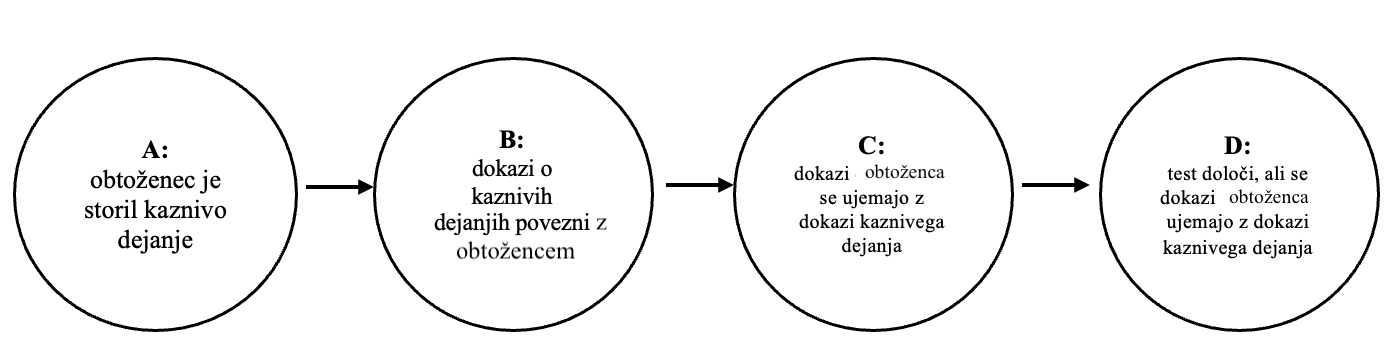
\includegraphics[scale=0.60]{slika_3.png}
    \caption{Vzorčna veriga dokazov}
 \end{figure}
 \\
\textit{Tožilčeva zmota}: pri tem enačimo $P(C \lvert \neg B)$ s $P(\neg A \lvert C)$. Presega napako predhodne verjetnosti, saj si jo lahko 
predstavljamo kot dopolnitev te napake z dodatno napačno predpostavko $P(A) = P(B)$.\\\\
\textit{Napaka verjetnosti $P(\text{drugo ujemanje})$}: gre za zmoto, ko verjetnost $P(C \lvert \neg B)$ enačimo z verjetnostjo
(imenujmo jo $q$), da ima vsaj en nedolžen član populacije ustreza dokazom. Posledica te napake je običajno močno pretiravanje z vrednostjo
dokaza $C$.\\\\
\textit{Zanemarjanje predhodnih verjetnosti}: to pomeni preprosto neupoštevanje predhodnih vrednosti, kot sta $P(A)$ in $P(B)$. Na splošno
se za zmoto zanemarjanja osnovne stopnje šteje, kadar je verjetnost dogodka podcenjena, ker dogodek ni tako nenavaden, kot se zdi,
ali precenjena, ker je dogodek bolj nenavaden, kot se zdi.\\\\
\textit{Napaka pri številčnem preračunavanju}: pri tem gre za zamenjavo vrednosti $P(C \lvert \neg B)$ s pričakovanim številom drugih oseb,
ki bi jih bilo treba testirati, preden bi našli ujemanje. Ta zmota prav tako pretirava z vrednostjo dokaza $C$.\\\\
\textit{Pričakovane vrednosti, ki pomenijo edinstvenost}: če je velikost populacije približno enaka $1/P(\neg B \lvert C)$, potem mora biti
obdolženec edini primerek. Binomski izrek pokaže, da obstaja več kot 25\% verjetnost, da bosta v populaciji, katere velikost je $1/P(\neg B \lvert C)$,
vsaj dva ujemanja.\\\\
\textit{Zmota obrambnega odvetnika}: to se zgodi, ko se dokaz $C$ šteje za nepomembnega, ker visoka predhodna verjetnost $P(\neg A)$ (kar
se zgodi, če je na primer potencialno število osumljencev zelo veliko) še vedno povzroči visoko verjetnost $P(\neg B \lvert C)$. \\\\
\textit{Napaka baze podatkov obrambnega odvetnika}: za to napako gre, kadar verjetnost $P(\neg B \lvert C)$ temelji na drugačni populaciji,
kot jo določa $P(B)$ ali $P(A)$.\\\\
\textit{Zasliševalčeva zmota}: v tem primeru je dokaz neposredno priznanje krivde. Če to ni potrjeno, to pomeni, da uporabljamo $P(D \lvert A)$ za
informiranje $P(A \lvert D)$. Napaka je, da ne upoštevamo $P(D \lvert \neg A)$. Če je $P(D \lvert A) \leq P(D \lvert \neg A)$, potem dokaz
nima vrednosti.\\\\
Poleg zmot, ki izhajajo iz osnovnega nerazumevanja pogojne verjetnosti, se druge zmote pojavijo zaradi neustreznega združevanja vpliva več dokazov:\\
\textit{Zmota odvisnih dokazov}: ta zmota, ki se včasih imenuje tudi dvojno štetje, se kaže v tem, da se dva ali več dokazov, ki so odvisni,
obravnava, kot da bi bili neodvisni, zaradi česar je izjava o njihovi skupni verjetnosti manjša, kot bi morala biti. Poseben primer te zmote je
\textit{logično odvisna dokazna zmota}, pri kateri en dokaz ni preprosto odvisen od drugega, ampak dejansko logično izhaja iz njega.\\\\
\textit{Napaka konjunkcije}: ta zmota se pojavi, kadar preiskovalec ne upošteva dejstva, da je dokaz sestavljen iz več kot enega negotovega dogodka,
in mu posledično pripiše večjo verjetnost, kot bi jo moral.

%%%%%%%%%%%%%%%%%%%%%%%%%%%%%%%%%%%%%%%%%%%%%%%%%%%%%%%%%%%%%%%%%%%%%%%%%%%%%%%%%%%%%%%%%%%%%%%%%%%%%%%%%%%%%%%%%%%%%%%%%%%%%%%%%%%%%%%%%%%%%%
\subsection{Tožilčeva zmota}
Verjetnostno utemeljevanje pravnih dokazov se torej skrči na preprost vzročni scenarij: začnemo z neko hipotezo $H$ in opazujemo nek dokaz $E$.
Poznavanje pogojne verjetnosti $P(E \lvert H)$ nam omogoča, da spremenimo svoje prepričanje o verjetnosti $H$, če poznamo $E$. Veliko najpogostejših
napak v sklepanju izhaja iz osnovnega nerazumevanja pogojne verjetnosti. Še posebej pogost primer je zamenjava verjetnost dokaza $E$ glede na
hipotezo $H$ z verjetnost hipoteze $H$ glede na dokaze $E$ oziroma $P(E \lvert H)$ z $P(H \lvert E)$, torej ko napačno verjamemo, da je verjetnost 
naključnega znanstvenega ujemanja enaka verjetnosti, da je obtoženec nedolžen. To se pogosto imenuje napaka prenesenega pogojnika oziroma tudi 
tožilčeva zmota.\\\\
Tožilčeva zmota se pogosto pojavlja v kazenskem pravu, vendar jo pogosto neprepoznajo, deloma zato, ker preiskovalci
nimajo močne intuicije o tem, kaj zmota sploh pomeni. Tožilčeva zmota je dobro znana statistična zmota, ki izhaja iz napačnega razumevanja
pogojnih verjetnosti in vprašanj večkratnega testiranja. Napaka temelji na predpostavki, da je $P(H \lvert E) = P(E \lvert H)$, pri čemer $H$
predstavlja primer, da se najdejo dokazi o obtožencu, $E$ pa primer, da je obtoženec nedolžen. Vendar ta enakost ne drži: čeprav je $P(H \lvert E)$
običajno zelo majhen, je lahko $P(E \lvert H)$ še vedno veliko večji. \\\\
Za lažjo predstavo si oglejmo primer. Naj se kri obtoženca ujema s krvjo storilca kaznivega dejanja. Ta krvna skupina je tako redka, 
da je verjetnost, da jo ima nekdo, le 1 proti 1000. Če si to statistiko razlagate tako, da obstaja le 1 proti 1000 možnosti, da je obtoženec 
nedolžen, ste žrtev tožilske zmote. Verjetnost naključnega ujemanja (pogostost krvnega profila) ste napačno združili z verjetnostjo vira (verjetnost, 
da je vir krvi nekdo drug kot obtoženec). V mestu z milijon prebivalci bi bilo približno 1000 ljudi z redkim krvnim profilom. Čeprav je torej 
res, da obstaja le verjetnost 1 proti 1000, da se kri naključne osebe ujema s krvjo zločinca, je verjetnost, da je oseba, ki ustreza redkemu 
profilu krvi, nedolžna, in sicer izključno na podlagi ujemanja dokazov, dejansko 999 proti 1000. \\\\
Do tožilčeve zmote lahko pride zaradi večkratnega testiranja, na primer pri primerjanju dokazov z veliko podatkovno bazo. Velikost podatkovne
zbirke povečuje verjetnost, da bo ujemanje ugotovljeno zgolj po naključju. \\\\
Če je $E$ dokaz in $H$ trditev,da je obtoženi nedolžen, upoštevamo pogojne verjetnosti: \\
$P(E \lvert H)$ \dots verjetnost resničnosti dokaz $E$, kljub temu da je obtoženi nedolžen; \\
$P(H \lvert E)$ \dots verjetnodt, da je obtoženi nedolžen kljub dokazu $E$. \\
Pri forenzičnih dokazih je ponavadi verjetnost $P(E \lvert H)$ majhna. Tožilec pa potem velikokrat sklepa, da je tudi verjetnost
$P(H \lvert E)$ majhna.
%(tožilstvo Lucie de Berk je na primer obtoženo ravno te napake)
Zgoraj napisani pogojni verjetnosti pa sta precej različni; uporabimo Bayesovo pravilo:
\[
   P(H \lvert E) = P(E \lvert H) \times \frac{P(H)}{P(E)}, \vspace{2mm}
\]
kjer je $P(H)$ verjetnost nedolžnosti in $P(E)$ verjetnost dokaza. Enačba kaže, da majhna pogojna verjetnost $P(E \lvert H)$ ne pomeni majhne
pogojne verjetnosti $P(H \lvert E)$ v primeru velike verjetnosti nedolžnosti in majhne verjetnosti dokaza. \\
Po Bayesovem pravilu je
\[
   P(E)=P(E \lvert H)P(H) + P(E \lvert \neg H)\times[1 - P(H)] \vspace{2mm}
\]
kjer je $P(E \lvert \neg H)$ verjetnost, da bodo dokazi identificirali krivega osumljenca; bičajno je ta verjetnost blizu 1.

\subsubsection{Primer - Tožilčeva zmota}
Slika 2 prikazuje populacijo 100 moških, starih 50 let, ki se ne zdravijo zaradi hipertenzije in imajo skupni holesterol 235 mg/dl in krvni tlak 120 mmHg. Pričakuje
se, da bo 9\% teh moških (predstavljeno z devetimi črtastimi kvadrati) čez 10 let imelo miokardni infarkt(MI). Ena četrtina moških je kadilcev (predstavljeno s 25
sivimi kvadrati); približno 16\% naj bi doživelo MI v 10 letih; zato bo $\frac{4}{25}$ kadilcev imelo MI (predstavljeno s črtastimi in sivimi kvadrati). \\
Število kadilcev, ki imajo MI, je očitno enako številu ljudi, ki imajo MI in so kadilci. Toda ali je delež kadilcev, ki imajo MI, enak deležu ljudi z MI, ki so kadilci? Iz
slike 2 je odogovor očitno ne; verjetnost, da ste kadilec glede na to, da ste imeli MI, torej:
\[
   P(\text{MI} \lvert \text{kadilec}) \ne P(\text{kadilec} \lvert \text{MI}), \vspace{2mm}
\]
ker
\[
   P(\text{MI} \lvert \text{kadilec}) = P(\text{črtasto} \lvert \text{sivo}) = \frac{4}{25} = 0,16 \vspace{2mm}
\]
in
\[
   P(\text{kadilec} \lvert \text{MI}) = P(\text{sivo} \lvert \text{črtasto}) = \frac{4}{9} = 0,44. \vspace{2mm}
\]
Vizualno opazimo, da delež sivih kvadratov, ki se prekrivajo s črtastimi kvadrati, ni enak deležu črtastih kvadratov, ki se prekrivajo s sivimi kvadrati.
\begin{figure}[!ht]\label{fig:slika1}
   \centering
   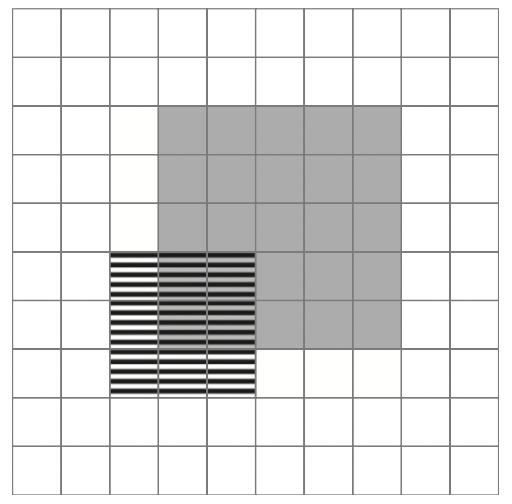
\includegraphics[scale=0.45]{slika1.png}
   \caption{Populacija, predstavljena s 100 kvadrati, z 9 črtastimi, 25 sivimi in 4 črtastimi in sivimi.}\vspace{2mm}
\end{figure}\\
Slika 3 prikazuje izjeme pri tožilčevi zmoti, predstavljeni na sliki 1. Sedaj imamo 16 črtastih kvadratov, 16 sivih in 4 pikčaste in sive kvadrate, ker je splošna
razširjenost črtastih in sivih kvadratov enaka, je
\[
   P(\text{črtasto} \lvert \text{sivo}) = P(\text{sivo} \lvert \text{črtasto}). \vspace{2mm}
\]
Tudi
\[
   P(\text{črtasto} \lvert \text{pikčasto}) = P(\text{pikčasto} \lvert \text{črtasto}), \vspace{2mm}
\]
saj sta obe verjetnosti enaki $0$. Oboje(podobno velike populacija in populacije brez prekrivanja) je ozka izjema zmote. \\
Po drugi strani pa so črtkani kvadrati na sliki 2 v celoti zajeti v sivih kvadratih; tako je
\[
   P(\text{sivo} \lvert \text{črtkano}) = 1, \quad \text{medtem ko je} \quad P(\text{črtkano} \lvert \text{sivo}) = 0,25. \vspace{2mm}
\]
Tožilčeva zmota velja, kadar je ena skupina podmnožica druge. 

\begin{figure}[!ht]\label{fig:slika2}
   \centering
   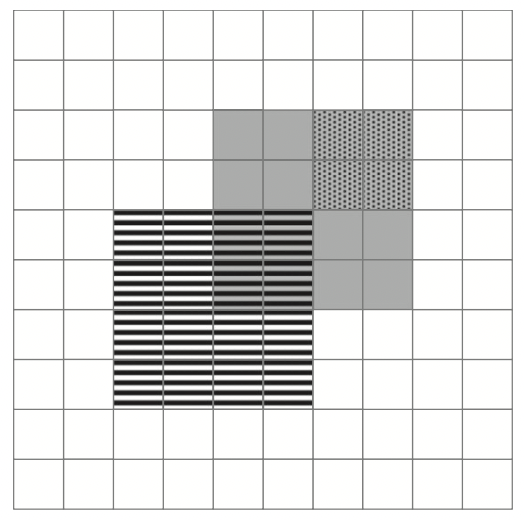
\includegraphics[scale=0.45]{slika2.png}
   \caption{Populacija, predstavljena s 100 kvadrati, z 16 črtastimi, 16 sivimi in 4 pikčastimi in sivimi.}\vspace{2mm}
\end{figure}

%%%%%%%%%%%%%%%%%%%%%%%%%%%%%%%%%%%%%%%%%%%%%%%%%%%%%%%%%%%%%%%%%%%%%%%%%%%%%%%%%%%%%%%%%%%%%%%%%%%%%%%%%%%%%%%%%%%%%%%%%%%%%%%%%%%%%%%%%%%%%%
%%%%%%%%%%%%%%%%%%%%%%%%%%%%%%%%%%%%%%%%%%%%%%%%%%%%%%%%%%%%%%%%%%%%%%%%%%%%%%%%%%%%%%%%%%%%%%%%%%%%%%%%%%%%%%%%%%%%%%%%%%%%%%%%%%%%%%%%%%%%%%
\section{Načini za izogib zmotam}
V zadnjih letih je statistika in verjetnost v kazenskem pravu napredovala. Sodniki, tožilstvo in porota se zavedajo nerazumevanja te znanosti, zato 
je statistika čedalje bolj vpletena že v učne programe pravnih fakultet, kar pripomore k boljšemu razumevanju statističnih analiz. Kljub temu so seveda 
zmote še vedno prisotne. V začetku dela sem omenila, da je razlaga statistične analize odvisna od vprašanj odvetnika, pri čemer veliko za izboljšanje 
ne moremo storiti. Poleg tega morajo biti statistični oziroma forenzični znanstveniki previdni z razlago, kajti ne smejo poseči v poroto. Torej kako 
se dejansko izognimo zmotam in s tem ne posežemo v pravna pravila na sodiščih. 

%%%%%%%%%%%%%%%%%%%%%%%%%%%%%%%%%%%%%%%%%%%%%%%%%%%%%%%%%%%%%%%%%%%%%%%%%%%%%%%%%%%%%%%%%%%%%%%%%%%%%%%%%%%%%%%%%%%%%%%%%%%%%%%%%%%%%%%%%%%%%%
\subsection{Izogib zmotam z uporabo razmerja verjetnosti}
Vsem zgoraj opisanim zmotam je skupno to, da je resnična koristnost dokaza predstavljena na zavajajoč način - bodisi je pretirana bodisi podcenjena.
Prednost uporabe razmerja verjetnosti je, da odpravlja ugovor Bayesovemu izreku, in sicer upoštevanje predhodne verjetnosti za hipotezo,
kot je »kriv«. V veliki meri pomiri pomisleke pravnikov, ki bi sicer zavrnili Bayesov argument z utemeljitvijo, da je nedopustno predpostavljati 
predhodne verjetnosti o krivdi ali nedolžnosti.\\\\
Čeprav je uporaba razmerja verjetnosti kot sredstva za izogibanje zmotam in merjenje uporabnosti dokazov močno podprta, sem vseeno mnenja, da
imajo, po prebiranju različnih sodb, pravniki in laiki pogosto podobne težave pri razumevanju razmerja verjetnosti kot pri razumevanju
Bayesove teorije.

%%%%%%%%%%%%%%%%%%%%%%%%%%%%%%%%%%%%%%%%%%%%%%%%%%%%%%%%%%%%%%%%%%%%%%%%%%%%%%%%%%%%%%%%%%%%%%%%%%%%%%%%%%%%%%%%%%%%%%%%%%%%%%%%%%%%%%%%%%%%%%
\subsection{Učinkovitost Bayesove teorije pri zmanjšanju zmote obrambnega odvetnika}
Zmota odvetnika je manj znana različica pogostejše tožilske zmote. Pri zmoti odvetnika je porota spodbujena, da asociativnih dokazov ne upošteva 
kot nepomembnih, ne glede na to, kako redka je značilnost ujemanja.\\
Za ponazoritev si predstavljajte sojenje z enakim ujemanjem krvi kot pri tožilčevi zmoti, vendar z dodatnimi dokazi proti obtožencu, kot sta 
očividec in posedovanje orodja za kaznivo dejanje. Zagovornik lahko kljub temu poroti pove, da je verjetnost obtoženčeve krivde le 1 proti 1000. 
To bi bilo sicer pravilno, če bi obtožnica utemeljevala primer samo na podlagi ujemanja krvi, vendar obrambni odvetnik dejansko prosi poroto, 
naj ne upošteva drugih dokazov razen ujemanja krvi. To je zmota obrambnega odvetnika. Če obrambnemu odvetniku uspe prepričati poroto, da verjame 
tej napačni logiki, lahko dodatni dokazi o ujemanju krvi napačno zmanjšajo verjetnost krivde pri poroti.\\
Čeprav so učinki tožilčeve zmote lahko hujši kot učinki zmote odvetnika (krivična obsodba v primerjavi s krivično oprostitvijo), so porote morda 
bolj dovzetne za slednjo kot za prvo. 

%%%%%%%%%%%%%%%%%%%%%%%%%%%%%%%%%%%%%%%%%%%%%%%%%%%%%%%%%%%%%%%%%%%%%%%%%%%%%%%%%%%%%%%%%%%%%%%%%%%%%%%%%%%%%%%%%%%%%%%%%%%%%%%%%%%%%%%%%%%%%%
\subsection{Učinkovitost Bayesove teorije pri zmanjšanju zasliševalčeve zmote}
To zmoto opredeljujemo kot zmoto, ki se kaže v tem, da izpovedni dokazi nikoli ne morejo zmanjšati verjetnosti krivde - v določenih okoliščinah 
lahko priznanje zmanjšal verjetnost krivde. Vprašanje je, kdaj natančno je priznanje znak krivde in kdaj ne. Priznanje poveča verjetnost krivde 
le, kadar je verjetnost priznanja, če je oseba kriva, večja od verjetnosti priznanja, če je oseba nedolžna. Če se $H$ nanaša na trditev, da je 
oseba kriva, $E$ pa na trditev, da oseba prizna, velja
\[
    P(H \lvert E) > P(H \lvert \neg E)
\]  
velja le pod pogojem, da je 
\[
    P(E \lvert H) > P(E \lvert \neg H).
\] 
\begin{trditev}
    Obstoj priznanja poveča verjetnost krivde, če in samo če je manj verjetno, da bo nedolžna oseba priznala kot kriva.
\end{trditev}
Slednjo trditev je mogoče izpeljati s pomočjo Bayesove teorije:
\begin{equation}\label{eq:btrditev}
    \frac{P(H \lvert E)}{P(\neg H \lvert E)} = \frac{P(H)}{P(\neg H)}  \times \frac{P(E \lvert H)}{P(E \lvert \neg H)}
\end{equation}
Na levi strani je \[\frac{P(H \lvert E)}{P(\neg H \lvert E)},\] razmerje posteriornih verjetnosti krivde in nedolžnosti (tj. verjetnosti po 
upoštevanju priznanja). Enak je zmnožku dveh drugih razmerij na desni strani. Razmerje \[\frac{P(H)}{P(\neg H)}\] predstavlja razmerje predhodnih 
verjetnosti krivde in nedolžnosti (to je verjetnosti krivde in nedolžnosti pred upoštevanjem dejstva priznanja). Zadnje razmerje, 
\[\frac{P(E \lvert H)}{P(E \lvert \neg H)},\] se imenuje razmerje verjetnosti in določa, kakšen vpliv bo imel nov dokaz (priznanje) na 
verjetnosti krivde in nedolžnosti. Zlasti bo posteriorna verjetnost krivde večja od predhodne verjetnosti krivde le, če bo razmerje verjetnosti 
večje od 1. Če pa je razmerje verjetnosti \[\frac{P(E \lvert H)}{P(E \lvert \neg H)} < 1,\] priznanje dejansko postane kazalnik nedolžnosti. \\\\
Ni nujno, da iz vsega tega sledi, da bi bil obstoj priznanja v tej situaciji dokaz proti krivdi. V nasprotju s tem, bi lahko priznanje še vedno 
povečalo verjetnost krivde, tudi če je bolj verjetno, da bo nedolžna oseba priznala kot kriva. Takšna zamisel se zdi logično nemogoča, če 
pogledamo \eqref{eq:btrditev}. Vendar želim povedati, da enačba \eqref{eq:btrditev} morda ni prava formula za uporabo v tem primeru. Morda obstaja še eno empirično dejstvo, 
ki je pomembno za verjetnost krivde. V tem primeru bi morali uporabiti bolj zapleteno formulo, ki bi vključevala to dejstvo. Ker tu preučujemo 
dokazni učinek priznanja, ki je rezultat zaslišanja, verjetnost, ki jo iščemo, v resnici ni verjetnost, da je oseba X kriva, če je priznala, 
ampak verjetnost, da je oseba X kriva, če je priznala in če je bila zaslišana. Zato je treba razmerje posteriornih verjetnosti izraziti na 
naslednji bolj celovit način, pri čemer $I$ predstavlja trditev »je bil zaslišan«:
\begin{equation}\label{eq:posteriorne}
    \frac{P(H \lvert E, I)}{P(\neg H \lvert E, I)} = \frac{P(H \lvert I)}{P(\neg H \lvert I)}  \times \frac{P(E \lvert H, I)}{P(E \lvert \neg H, I)}
\end{equation}
in z nadaljnjo razširitvijo prvega razmerja verjetnosti na desni strani \eqref{eq:posteriorne}
\begin{equation}\label{eq:razširitev}
    \frac{P(H \lvert E, I)}{P(\neg H \lvert E, I)} = \frac{P(H)}{P(\neg H)} \times \frac{P(I \lvert H)}{P(I \lvert \neg H)}  \times \frac{P(E \lvert H, I)}{P(E \lvert \neg H, I)}
\end{equation}
Da bi videli, zakaj je prvo razmerje na desni strani \eqref{eq:posteriorne} enakovredno produktu prvih dveh razmerij na desni strani \eqref{eq:razširitev}, najprej upoštevajmo naslednji dve osnovni verjetnostni resnici:
\begin{equation}\label{eq:ver1}
    P(H \lvert I) = \frac{P(H) \times P(I \lvert H)}{P(I)}
\end{equation}
\begin{equation}\label{eq:ver2}
    P(\neg H \lvert I) = \frac{P(\neg H) \times P(I \lvert \neg H)}{P(I)}
\end{equation}
Če zdaj \eqref{eq:ver1} delim z \eqref{eq:ver2} dobim
\begin{equation}\label{eq:enakovredno}
    \frac{P(H \lvert I)}{P(\neg H \lvert I)} = \frac{P(H)}{P(\neg H)}  \times \frac{P(I \lvert H)}{P(I \lvert \neg H)}
\end{equation}
Enačba \eqref{eq:enakovredno} dokazuje, da sta \eqref{eq:posteriorne} in \eqref{eq:razširitev} enakovredni.\\\\
Primerjajmo enačbo \eqref{eq:btrditev} z enačbo \eqref{eq:razširitev}, ki daje popolnejšo sliko stanja. Na levi strani je v vsakem primeru razmerje posteriornih verjetnosti krivde in nedolžnosti, s to 
razliko, da so v \eqref{eq:btrditev} te verjetnosti pogojene samo s priznanjem, medtem ko so v \eqref{eq:razširitev} pogojene tako s priznanjem kot z zaslišanjem. Prvo razmerje na desni strani je enako 
tako v \eqref{eq:btrditev} kot \eqref{eq:razširitev}: razmerje predhodnih verjetnosti $H$ in $\neg H$. Tudi zadnje razmerje na desni strani je v obeh primerih podobno: verjetnost priznanja glede na 
krivdo (in zaslišanje), deljena z verjetnostjo priznanja glede na nedolžnost (in zaslišanje). V enačbi \eqref{eq:razširitev} imamo na desni strani razmerje 
\[\frac{P(I \lvert H)}{P(I \lvert \neg H)},\] kar je verjetnost, da vas bo policija zaslišala, če je oseba kriva, deljena z verjetnostjo, da vas bo policija 
zaslišala, če je oseba nedolžna. To razmerje je večje od 1. Razumno je namreč pričakovati, da bo policija z večjo verjetnostjo izbrala za zaslišanje nekoga, 
ki je kriv, kot nekoga, ki je nedolžen. Prav to razmerje v \eqref{eq:razširitev} razkriva, kaj je narobe z zgornjo trditvijo, da se lahko verjetnost krivde po priznanju poveča le, 
če je $P(E \lvert H) > P(E \lvert \neg H)$. \\
To lahko pokažemo s preprostim protiprimerom. Sprejmimo domnevo, da kriminalci pod policijskim nadzorom redkeje priznajo kot nedolžni ljudje. Recimo, da prizna 
le 40 odstotkov krivcev, medtem ko prizna 60 odstotkov nedolžnih. Ker je zaradi tega verjetnost priznanja glede na krivdo manjša od verjetnosti priznanja glede 
na nedolžnost, se zdi, da sledi, da zdaj obstoj priznanja ne more povečati verjetnosti krivde od tiste, ki je bila pred priznanjem. Toda predpostavimo še, 
da je verjetnost, da bo policija zaslišala krivega, devetkrat večja kot verjetnost, da bo zaslišala nedolžnega posameznika. Nazadnje predpostavimo, da je 
predhodna verjetnost, da je oseba X kriva, na podlagi vseh dokazov pred priznanjem, 0,75. \\
Verjetnosti, ki veljajo za opisano situacijo:\\ \vspace{2mm}
$P(E \lvert H, I) = 0,4\\ \vspace{2mm}$
$P(E \lvert \neg H, I) = 0,6\\ \vspace{2mm}$
$P(H) = 0,75\\ \vspace{2mm}$
$P(\neg H) = 0.25\\ \vspace{2mm}$
$\frac{P(I \lvert H)}{P(I \lvert \neg H)} = 9.\\ \vspace{2mm}$
Sledi po enačbi \eqref{eq:razširitev}
\begin{equation}\label{eq:rezultat}
    \frac{P(H \lvert E, I)}{P(\neg H \lvert E, I)}  = \frac{P(H \lvert I)}{P(\neg H \lvert I)}  \times \frac{P(E \lvert H, I)}{P(E \lvert \neg H, I)} = \frac{0,75}{0,25} \times 9 \times \frac{0,4}{0,6} = 18
\end{equation}
Enačba \eqref{eq:rezultat} nam pove, da je verjetnost, da je oseba X kriva, ob upoštevanju vseh okoliščin, 18-krat večja od verjetnosti, da je nedolžena. Ker mora biti 
bodisi kriva bodisi nedolžena, lahko to razmerje uporabimo za pridobitev posteriorne verjetnosti krivde osebe X. Verjetnost, da je kriva, glede na to, 
da je priznala (in da je bil zaslišana), je 18/19 ali 0,95. Pred priznanjem je bila verjetnost krivde 0,75. Po priznanju se verjetnost krivde poveča 
na 0,95 kljub temu, da je verjetnost, da bo priznala, če je kriva, manjša od verjetnosti, da bo priznala, če je nedolžena. \\
S tem je dokaz, da je priznanje lahko dokaz krivde le, če je verjetnost priznanja glede na krivdo večja od verjetnosti priznanja glede na nedolžnost, popoln.

%%%%%%%%%%%%%%%%%%%%%%%%%%%%%%%%%%%%%%%%%%%%%%%%%%%%%%%%%%%%%%%%%%%%%%%%%%%%%%%%%%%%%%%%%%%%%%%%%%%%%%%%%%%%%%%%%%%%%%%%%%%%%%%%%%%%%%%%%%%%%%
%%%%%%%%%%%%%%%%%%%%%%%%%%%%%%%%%%%%%%%%%%%%%%%%%%%%%%%%%%%%%%%%%%%%%%%%%%%%%%%%%%%%%%%%%%%%%%%%%%%%%%%%%%%%%%%%%%%%%%%%%%%%%%%%%%%%%%%%%%%%%%
\section{Nadaljevanje kazenskega primera - medicinska sestra Lucia de Berg: Interpretacija verjetnosti na sodišču}
Sodišče je bilo mnenja, da verjetnostni izračun, ki ga je podal Henk Elfferson, pomeni, da je osumljenka vse dogodke, navedene v obtožnici, doživela naključno. Ti 
izračuni naj bi poseldično prikazovali, da je velika verjetnost, da obstaja povezava med izmeno osumljenke in pojavom incidenta. Te sklepi sodišča bi morali statistikom 
vzbujati dvome, saj se sodba dvoumna in lahko bi rekla, da je sodišče storilo znano tožilčevo zmoto. Po sklepu sodišča bi lahko rekli, da govorijo o verjetnosti, da se je nekaj zgodilo 
ob predpostavki, da je vse popolnoma naključno ali pa si sodbo sodišča razlagamo kot verjetnost, da se je nekaj naključno zgodilo. Te dve trditvi pa sta različni, kar lahko 
pokažem z naslednjimi formulami. Naj bo\\
$F$ \dots opazovani dogodek;\\
$H_0$ \dots trditev, da se dogodek zgodi naključno.\\
Henk Elffers je izračunal verjetnost $P(F \lvert H_0) < 342 \times 10^{-6}$, medtem ko je sodišče mislilo, da je Elffersonova izračunana  verjetnost v bistvu $P(H_0 \lvert F)$, 
kar pa je definicija tožilčeve zmote.\\\\
Torej poleg tega, da je bila uporabljena metoda za izračun verjetnosti nekoliko sporna, kljub kasnejšim popravkom, je na koncu prišlo še do napake na sodišču, zaradi 
nerazumevanja pogojnih verjetnosti. Če bi hoteli pravično sodbo, bi, po mojem mnenju, seveda morali najprej izbrati ustrezne metode za izračun vseh verjetnosti, predstavitev 
statistične analize na sodišču pa bi morala biti bolj temeljita in prilagojena razumevanju sodnikom, odvetnikom in poroti. Sodba se je kasneje ponovno odprla, 
zaradi ugovorov na uporabljene metode Henka Elffersona.

%%%%%%%%%%%%%%%%%%%%%%%%%%%%%%%%%%%%%%%%%%%%%%%%%%%%%%%%%%%%%%%%%%%%%%%%%%%%%%%%%%%%%%%%%%%%%%%%%%%%%%%%%%%%%%%%%%%%%%%%%%%%%%%%%%%%%%%%%%%%%%
%%%%%%%%%%%%%%%%%%%%%%%%%%%%%%%%%%%%%%%%%%%%%%%%%%%%%%%%%%%%%%%%%%%%%%%%%%%%%%%%%%%%%%%%%%%%%%%%%%%%%%%%%%%%%%%%%%%%%%%%%%%%%%%%%%%%%%%%%%%%%%
\section{Izogibanje zmotam z uporabo Bayesovih \\omrežij}
Ker je največkrat težava v tem, da se večina odvetnikov in sodnikov ob pogledu na verjetnostne izračune in statistično analizo dokazov, ustraši, se mi 
zdijo Bayeosova omrežja dober predlog za predstavitev verjetnostnih izračunov.

%%%%%%%%%%%%%%%%%%%%%%%%%%%%%%%%%%%%%%%%%%%%%%%%%%%%%%%%%%%%%%%%%%%%%%%%%%%%%%%%%%%%%%%%%%%%%%%%%%%%%%%%%%%%%%%%%%%%%%%%%%%%%%%%%%%%%%%%%%%%%%
\subsection{Opredelitev}
Bayesova omrežja pomagajo določiti ustrezne verjetnostne formule, ne da bi prikazali njihovo polno algebrsko obliko, in omogočajo
skoraj popolno avtomatizacijo potrebnih verjetnostnih izračunov.
\begin{definicija}
   Bayesovo omrežje je verjetnostni grafični model, ki predstavlja množico spremenljivk in njihovih pogojnih odvisnosti prek usmerjenega
   acikličnega grafa.
\end{definicija}
Vozlišča teh usmerjenih acikličnih grafov predstavljajo spremenljivke (lahko so opazovane količine, latentne spremenljivke, neznani parametri
ali hipoteze). Povezave predstavljajo pogojne odvisnosti; vozlišča, ki niso povezana, predstavljajo spremenljivke, ki so pogojno neodvisne
druga od druge. Vsako vozlišče je povezano z verjetnostno funkcijo, ki kot vhodni podatek sprejme določen niz vrednosti za nadrejene spremenljivke
vozlišča in kot izhodni podatek poda verjetnost (ali verjetnostno porazdelitev, če je primerno) spremenljivke, ki jo predstavlja vozlišče. Puščice
predstavljajo razmerja pomembnosti, ki jih strokovnjak predvideva v okviru zadevnega problema sklepanja. Usmerjena povezava od vozlišča A do
vozlišča B pomeni, da ima A neposreden vpliv na B. Povezave med vozlišči se včasih razlagajo kot vzročne povezave, vendar opredelitev Bayesovih
omrežij ne zahteva, da povezave predstavljajo vzročni vpliv. Na splošno velja, da povezave v omrežju predstavljajo verjetnostna razmerja
pomembnosti. Značilnost Bayesovih omrežij je vključitev verjetnosti v obliki tabel, povezanih z vsakim vozliščem. To omogoča razlago narave in
moči odnosov med različnimi grafičnimi komponentami omrežja. Tabele verjetnosti vozlišč lahko torej obravnavamo kot sredstvo za povezovanje
modela s podatki.

%%%%%%%%%%%%%%%%%%%%%%%%%%%%%%%%%%%%%%%%%%%%%%%%%%%%%%%%%%%%%%%%%%%%%%%%%%%%%%%%%%%%%%%%%%%%%%%%%%%%%%%%%%%%%%%%%%%%%%%%%%%%%%%%%%%%%%%%%%%%%%
\subsection{Uporaba Bayesovih omrežij na sodišču}
Bayesova omrežja, ki temeljijo na Bayesovi teoriji in teoriji grafov, ponujajo forenzičnim znanstvenikom več prefinjenih možnosti. Tem metodam
se daje poseben poudarek, kadar je treba med konkurenčnimi hipotezami izbrati najverjetnejšo, izbira pa mora biti podprta z znanstveno utemeljeno
argumentacijo. Primerna so za analizo dogodka, ki se je zgodil, in napovedovanje verjetnosti, da je k temu prispeval katerikoli od več možnih
znanih vzrokov. Prednosti Bayesovih mrež se najbolj izrazito pokažejo na zapletenih področjih z več spremenljivkami. Kriminalistične aplikacije
Bayesovih omrežij segajo od prepoznavanja storilcev, posameznih in kompleksnih konfiguracij različnih vrst sledi ter problemov sklepanja, ki
vključujejo rezultate analiz DNK.\\
Ti grafični modeli verjetnosti bistveno izboljšajo vrednotenje verjetnostnih razmerij, ki se uporabljajo za ocenjevanje znanstvenih dokazov.
Omogočajo, da se lotimo kompleksnejših verjetnostnih analiz, kot bi bilo to mogoče s tradicionalnimi pristopi, kar še posebaj pride prav pri primerih z ogromno doazi. \\\\
Struktura Bayesovega omrežja v pravnem kontekstu je dovzetna za napačne predpostavke in napake v procesu ustvarjanja. Izbira vozlišč za dokaze je lahko
pristranska glede na to, kakšna vrsta argumenta je predstavljena. Argumenti obrambe ali tožilstva lahko na primer poudarjajo nasprotne sklepe
in zato vključujejo le podskupino dokazov. Če se za izdelavo ne uporablja dosleden okvir, lahko Bayesovo omrežje, ki jih oblikujejo različne stranke za en
primer, kažejo različne rezultate. Pri oblikovanju Bayesovega omrežja za pravno sklepanje ključnega pomena, da se oblikuje omrežje, ki je razumljivo poroti
in sodniku.\\\\
Prikaz Bayesovega omrežja se mora ujemati z intuitivnim pripisovanjem vzročno-posledičnih povezav med končno hipotezo, kot je »Obtoženec je kriv.«, podhipotezo
»Obtoženec je bil na kraju zločina.« in dokazi primera. Poleg težav, ki se pojavijo med postopkom strukturiranja, je problematično tudi sklepanje
iz omrežja, če se izvaja ob napačnih predpostavkah. Verjetnosti, tudi če temeljijo na strokovni presoji, so lahko pristranske zaradi dejavnikov
motenj v postopku pridobivanja podatkov. Metode za sklepanje morajo zato zagotoviti, da se verjetnosti omrežij ne razlagajo napačno kot dejstva in
da se izpostavi dejavnik negotovosti. Primerjati morajo verjetnosti za nasprotujoče si hipoteze in morajo zagotoviti okvir za pravnike, da iz
mreže sklepajo na argumente.

\section{Zaključek}

%%%%%%%%%%%%%%%%%%%%%%%%%%%%%%%%%%%%%%%%%%%%%%%%%%%%%%%%%%%%%%%%%%%%%%%%%%%%%%%%%%%%%%%%%%%%%%%%%%%%%%%%%%%%%%%%%%%%%%%%%%%%%%%%%%%%%%%%%%%%%%
\begin{thebibliography}{99}
    \bibitem{referenca-clanek}
        C. Aitken, G. Jackson in P. Roberts, \emph{1. Fundamentals of Probability and Statistical Evidence in Criminal Proceedings}, Guidance for Judges, Lawyers, Forensic Scientists and Expert Witnesses, Communicating and Interpreting Statistical Evidence in the Administration of Criminal Justice, 2010.

    \bibitem{referenca-clanek}
        C. Aitken in Y. McDermott, \emph{Analysis of evidence in international criminal trials using Bayesian Belief Networks}, Law, Probability and Risk, \textbf{16} (2017) 111-129.

    \bibitem{referenca-clanek}
        C. Aitken, W. C. Thompson in F. Taroni, \emph{How the Probability of a False Positive Affects the Value of DNA Evidence}, J. Forensic Sci., \textbf{48} (2003) 47-54.

    \bibitem{referenca-clanek}
        D. Balding, N. Fenton, R. Gill, D. Lagnado in L. Schneps \emph{Twelve Guiding Principles and Recommendations for Dealing with Quantitative Evidence in Criminal Law}, Probability and Statistics in Forensic Science,Isaac Newton Institute for Mathematical Sciences, 2017.

    \bibitem{referenca-clanek}
        D. Berger, N. Fenton in M. Neil, \emph{Bayes and the Law}, Annu Rev Stat Appl. Author manuscript., \textbf{3} (2016) 51-77.

    \bibitem{referenca-clanek}
        M. Conklin, \emph{The Effectiveness of Bayesian Jury Instructions in Mitigating the Defense Attorney's Fallacy}, Hous. L. Rev., \textbf{73} (2019) 21-30.

    \bibitem{referenca-clanek}
        M. Collins, R. Gill, M. Van Lambalgen in R. Meester, \emph{On the (ab)use of statistics in the legal case against the nurse Lucia de B.}, Law, Probability and Risk, \textbf{5} (2007) 233-250.

    \bibitem{referenca-clanek}
        C. Dahlman in E. Kolflaath, \emph{The Problem of the Prior in Criminal Trials}, Lund University in University of Bergen, 2021.

    \bibitem{referenca-clanek}
        N. Fenton in M. Neil, \emph{Avoiding Probabilistic Reasoning Fallacies in Legal Practice using Bayesian Networks}, RADAR, School of Electronic Engineering and Computer Science, Queen Mary (University of London), 2008.

    \bibitem{referenca-clanek}
        N. Fenton in M. Neil, \emph{The “Jury Observation Fallacy” and the use of Bayesian Networks to present Probabilistic Legal Arguments}, Oddelek za računalništvo in informatiko, Faculty of Informatics and Mathematical Sciences, Queen Mary and Westfield College, 2000.

    \bibitem{referenca-clanek}
        J. L. Gastwirth, \emph{Statistical Reasoning in the Legal Setting}, The American Statistician, \textbf{46} (1992) 55–69.

    \bibitem{referenca-clanek}
        A. Giannini, \emph{Theories of Evaluation of Evidence and the International Criminal Court Practice}, Maastricht University - Department of Criminal Law and Criminology, 2017.

    \bibitem{referenca-clanek}
        N. Iliinsky in D. Westreich, \emph{Epidemiology Visualized: The Prosecutor’s Fallacy}, American Journal of Epidemiology, \textbf{179} (2014) 1125-1127.

    \bibitem{referenca-clanek}
        C. de Macedo, \emph{Guilt by statistical association: revisiting the prosecutor’s fallacy and the interrogator’s fallacy}, The Journal of Philosophy, \textbf{105} (2008) 320-332.

    \bibitem{referenca-clanek}
        R. A. Matthews, \emph{The interrogator’s fallacy}, Aston University, 1995.

    \bibitem{referenca-clanek}
        J. Orbán, \emph{Bayesian Networks in Law Enforcement}, Budapest University of Technology and Economics, 2022.

    \bibitem{referenca-clanek}
        E. L. Schumann in W. C. Thompson, \emph{Interpretation of Statistical Evidence in Criminal Trials}, Law and Human Behavior, \textbf{11} (1987) 167–187.

    \bibitem{referenca-clanek}
        E. L. Schumann in W. C. Thompson, \emph{Interpretation of statistical evidence in criminal trials - The Prosecutor's Fallacy and the Defense Attorney's Fallacy}, Law and Human Behavior, \textbf{11} (1987) 167-187.

    \bibitem{referenca-clanek}
        N. Scurich, \emph{Interpretative Arguments of Forensic Match Evidence: An Evidentiary Analysis}, University of Southern California, 2010.

    \bibitem{referenca-clanek}
        R. Tarling, \emph{Statistical applications in criminology}, The Statisticia. \textbf{35} (1986) 369-388.

    \bibitem{referenca-knjiga}
        C. Aitken, S. Bozza in F. Taroni, \emph{Evidence for Forensic Scientists}, \textbf{3}, Wiley, West Sussex, 2021.

    \bibitem{referenca-knjiga}
        M. B. Blankenship in G. F. Vito, \emph{Statistical analysis in criminal justice and criminology: a user's guide}, \textbf{1}, Prentice Hall, Upper Saddle River, 2002.

    \bibitem{referenca-knjiga}
        B. Byers in J. McKean, \emph{Data analysis for criminal justice and criminology: practice and applications}, \textbf{1}, Allyn and Bacon, Boston, 2000.

    \bibitem{referenca-knjiga}
        M. O. Finkelstein in B. Levin, \emph{Statistics for Lawyers - Statistics for Social and Behavioral Sciences}, \textbf{3}, Springer, New York, 2015.

    \bibitem{referenca-knjiga}
        P. D. Hoff, \emph{A First Course in Bayesian Statistical Methods}, \textbf{1}, Springer, New York, 2009.

    \bibitem{referenca-knjiga}
        S. Maddan in J. T. Walker, \emph{Statistics in criminology and criminal justice: analysis and interpretation}, \textbf{3}, Jones and Bartlett Publishers, Sudbury, 2009.

    \bibitem{referenca-knjiga}
        B. Marcot, P. Naim in O. Pourret, \emph{Bayesian Networks, A Practical Guide to Applications}, \textbf{1}, John Wiley \& Sons, West Sussex, 2008.

    \bibitem{diploma-magisterij}
        M. Di Bello, \emph{Statistics and probability in criminal trials}, doktorska dizertacija, Oddelek za filozofijo, Univerza Stanford, 2013.

    \bibitem{referenca-spletni-vir}
        J. Balaba, \emph{Statistical Analysis In Criminal Justice Research}, v: Journal of Civil and Legal Sciences, 5, [3. december 2022], dostopno na \url{https://www.omicsonline.org/open-access/statistical-analysis-in-criminal-justice-research}.

    \bibitem{referenca-spletni-vir}
        A. Biedermann, F. Taroni, W. C. Thompson in J. Vuille, \emph{The role of prior probability in forensic assessments}, v: Front Genet., 3, [15. oktober 2022], dostopno na \url{https://www.ncbi.nlm.nih.gov/pmc/articles/PMC3809556/}.

    \bibitem{referenca-spletni-vir}
        D. A. Glover in V. Ramakrishnan, \emph{The use of statistics in legal proceedings: a primer for courts}, v: The Royal Society, 1, [25. november 2022], dostopno na \url{royalsociety.org/science-and-law}.

    \bibitem{referenca-spletni-vir}
        W. P. Skorupski in H. Wainer, \emph{The Bayesian flip: Correcting the prosecutor's fallacy}, v: Royal Statistical Society, 4, [22. oktober 2022], dostopno na \url{https://rss.onlinelibrary.wiley.com/doi/full/10.1111/j.1740-9713.2015.00839.x}.

\end{thebibliography}


\end{document}
